\section{Versão Alfa}
\subsection{Teste Unitário - Artigo}
\indent \par Na legislação, em determinado artigo está definido o tempo de espera para o código processual em questão,bem como a contagem de férias e dias não uteis. Desta forma, optamos por construir o nosso artigo com os seguintes atributos:
\indent \par - IdCodigo: ID de um determinado código
\indent \par - NrArtigo: Número do artigo a que correspondem os dados inseridos
\indent \par - IdUtilizador: ID do utilizador a que corresponde determinado artigo
\indent \par - Nome: Nome atribuido ao artigo pelo utilizador
\indent \par - Dias: Número de dias correspondente ao artigo
\indent \par - Meses: Número de meses correspondente ao artigo
\indent \par - Anos: Número de anos correspondente ao artigo
\indent \par - Ferias: True caso o artigo contabilize as férias, false caso contrário
\indent \par - DiasNaoUteis: True caso o artigo contabilize os dias não uteis, falso caso contrário

\begin{figure}[!h]
\centering
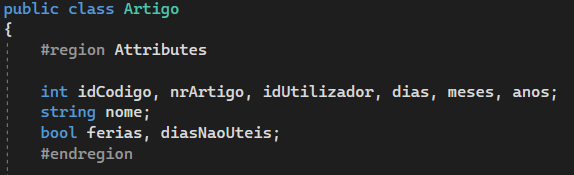
\includegraphics[width=0.8\textwidth]{Figuras/Models/ArtigoModel.png}
\caption{Artigo Model}
\label{d.model}
\end{figure}

\indent \par Em relação aos casos de uso, definimos que um utilizador seria capaz de inserir, alterar, eliminar artigos, bem como conseguir listar todos os artigos inseridos, ou, os artigos inseridos por determinado código processual.
\indent \par Procedemos então aos testes unitários para cada um destes casos de uso.
\indent \par Na inserção, criamos uma instância de um artigo com dados de teste e tentamos inseri-lo num determinado utilizador. O resultado obtido foi de acordo com o esperado.
\indent \par Na alteração de um artigo, pegamos nos atributos do artigo de teste criado anteriormente e procedemos à alteração de atributos. Obtivemos novamente sucesso no teste criado.
\indent \par Em relação à remoção de um artigo, tentamos eliminar o artigo de teste e o resultado foi, também, positivo.
\indent \par Na listagem de artigos, primeiro tentamos obter os artigos por número de utilizador e, por fim, tentamos a consulta de artigos por utilizador e por código processual. Ambos os testes correram como esperado.

\begin{figure}[!htbp]
  \centering
  \begin{minipage}[b]{0.4\textwidth}
    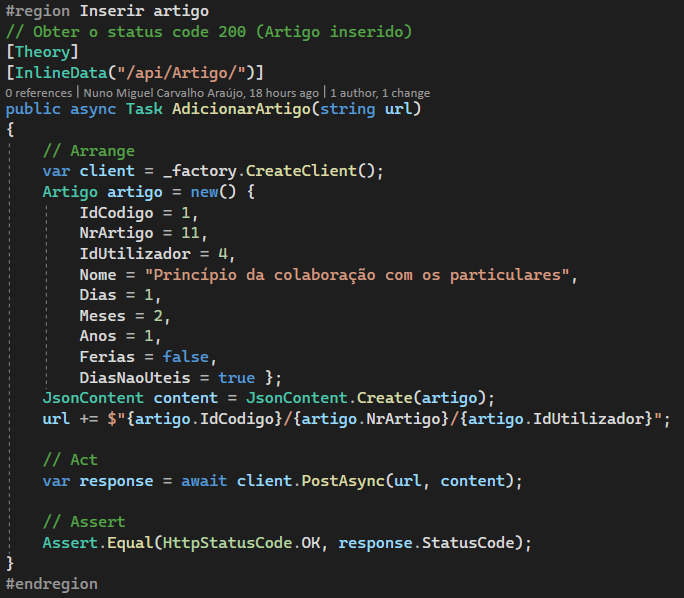
\includegraphics[width=\textwidth]{Figuras/TestesUnitarios/Artigo/Inserir Artigo.png}
    \caption{Inserir Artigo}
    \label{d.unitario}
  \end{minipage}
  \hfill
  \begin{minipage}[b]{0.4\textwidth}
    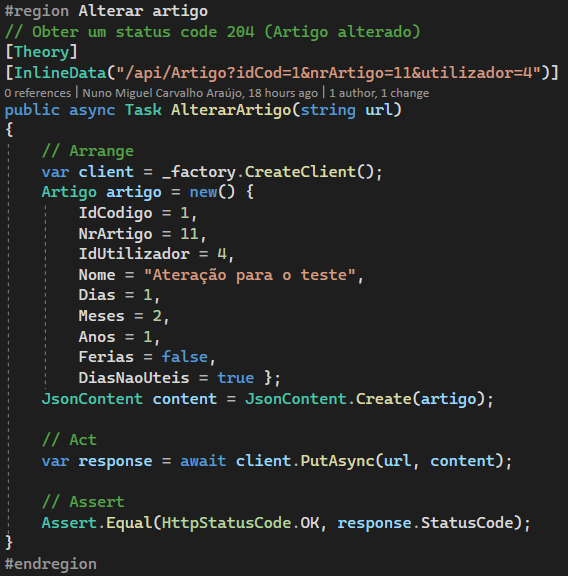
\includegraphics[width=\textwidth]{Figuras/TestesUnitarios/Artigo/Alterar Artigo.png}
    \caption{Alterar Artigo}
    \label{d.unitario}
  \end{minipage}
  \centering
  \begin{minipage}[b]{0.4\textwidth}
    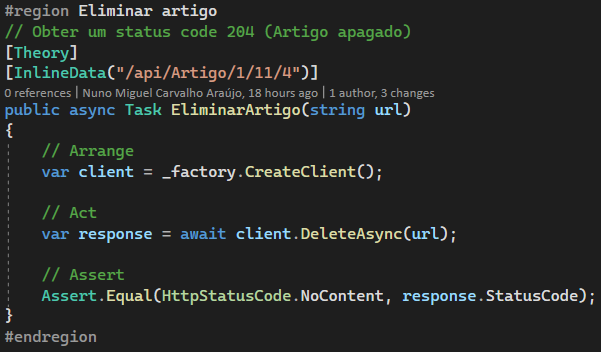
\includegraphics[width=\textwidth]{Figuras/TestesUnitarios/Artigo/Eliminar Artigo.png}
    \caption{Eliminar Artigo}
    \label{d.unitario}
  \end{minipage}
  \hfill
  \begin{minipage}[b]{0.4\textwidth}
    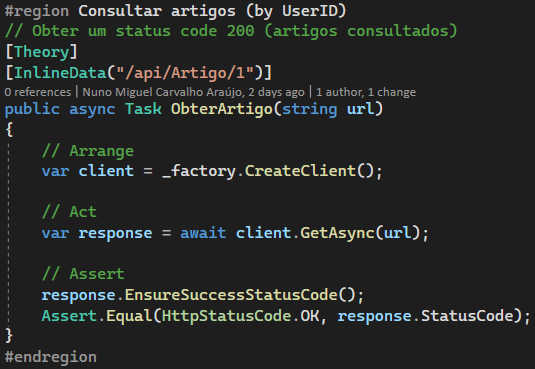
\includegraphics[width=\textwidth]{Figuras/TestesUnitarios/Artigo/Consultar artigos (by UserID).png}
    \caption{Consultar Artigo (by UserID)}
    \label{d.unitario}
  \end{minipage}
  \begin{minipage}[b]{0.4\textwidth}
    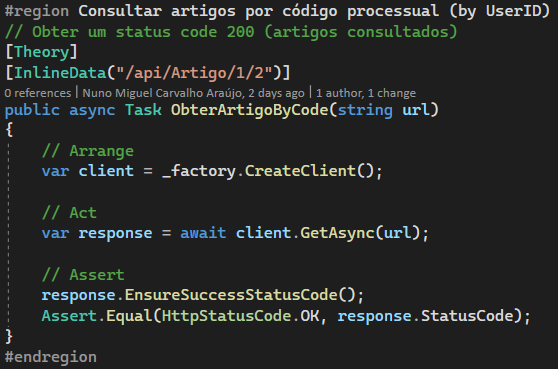
\includegraphics[width=\textwidth]{Figuras/TestesUnitarios/Artigo/Consultar artigos por código processual (by UserID).png}
    \caption{Consultar Artigos por Código Processual (by UserID)}
    \label{d.unitario}
  \end{minipage}
\end{figure}

\begin{figure}[!h]
\centering
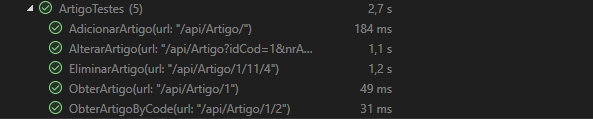
\includegraphics[width=1\textwidth]{Figuras/Testes/ArtigoTestes.png}
\caption{Artigo Testes}
\label{d.teste}
\end{figure}

\newpage


\subsection{Teste Unitário - Codigo}
\indent \par Pretendíamos obter uma listagem genérica dos códigos processuais, desta forma, criamos um objeto um objeto para satisfazer essas necessidades. Assim sendo, o código tem os seguintes atributos:
\indent \par - Id: ID para identificação do código noutros objetos
\indent \par - Nome: Descriminação juridica de um código (procedimento administrativo, processo cívil, processo penal e regime ilicito de mera ordenação social)

\begin{figure}[!h]
\centering
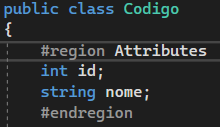
\includegraphics[width=0.4\textwidth]{Figuras/Models/CodigoModel.png}
\caption{Código Model}
\label{d.model}
\end{figure}

\indent \par Como estamos a falar de uma classe com uma listagem genérica, apenas permitimos a consulta dos códigos processuais inseridos em base de dados, assim sendo, testamos a obtenção desta lista. O teste correu conforme as expectativas.

\begin{figure}[!h]
\centering
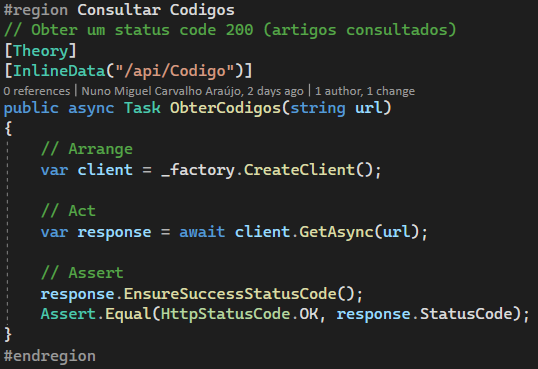
\includegraphics[width=0.4\textwidth]{Figuras/TestesUnitarios/Codigo/Consultar Codigos.png}
\caption{Consultar Codigos}
\label{d.unitario}
\end{figure}

\begin{figure}[!h]
\centering

\includegraphics[width=1\textwidth]{Figuras/Testes/CodigoTestes.png}
\caption{Código Testes}
\label{d.teste}
\end{figure}

\newpage


\subsection{Teste Unitário - Estado}
\indent \par Assim como o Código, o estado armazena uma listagem genérica de estados de uma fase processual. Sendo assim, criamos o estado com os seguintes atributos:
\indent \par - Id: ID para a identificação do estado noutros objetos
\indent \par - Nome: Descriminação de um estado (Fase articulados, fase de instrução e fase decisória)

\begin{figure}[!h]
\centering
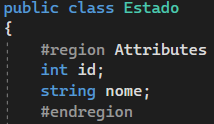
\includegraphics[width=0.4\textwidth]{Figuras/Models/EstadoModel.png}
\caption{Estado Model}
\label{d.model}
\end{figure}

\indent \par Falando, novamente, de uma listagem genérica, apenas testamos a obtenção da lista dos estados existentes. O teste foi de encontro às expectativas.

\begin{figure}[!h]
\centering
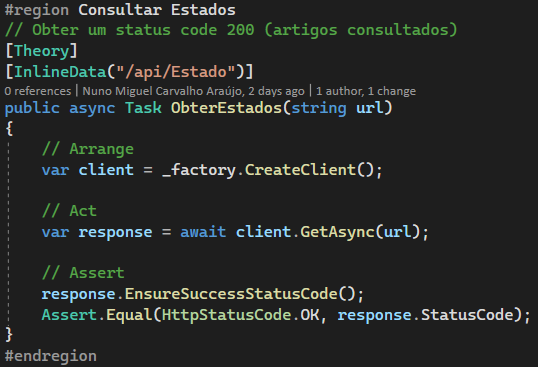
\includegraphics[width=0.4\textwidth]{Figuras/TestesUnitarios/Estado/Consultar Estados.png}
\caption{Consultar Estados}
\label{d.unitario}
\end{figure}

\begin{figure}[!h]
\centering

\includegraphics[width=1\textwidth]{Figuras/Testes/EstadoTestes.png}
\caption{Código Testes}
\label{d.teste}
\end{figure}

\newpage


\subsection{Teste Unitário - Fase Processual}
\indent \par Uma fase processual regista o tempo que o respetivo processo esteve em determinada fase. Existem três fases: fase articulados, fase de instrução e fase decisória. Cada processo só pode passar uma vez por cada uma destas fases e só pode mudar para a fase seguinte se a fase anterior já estiver terminada. Não existe ordem definida na passagem de um processo pelas diferentes fazes.
\indent \par Para conseguir garantir o bom funcionamento da fase processual, criamos a estrutura com os seguintes atributos:
\indent \par - IdUtilizador: ID para identificação do utilizador a que pertence a fase. (nota: o utilizador já deverá ter registado o processo para lhe atribuir uma fase)
\indent \par - IdEstado: ID que identifica qual a fase em que o processo se encontra
\indent \par - NrProcesso: Número do processo a que a fase processual está atribuída
\indent \par - DataEntrada: Data de entrada do processo em determinada fase processual
\indent \par - DataSaida: Data de saída do processo em determinada fase processual
\indent \par - NrDias: Número de dias em que o processo esteve em determinada fase processual

\begin{figure}[!h]
\centering
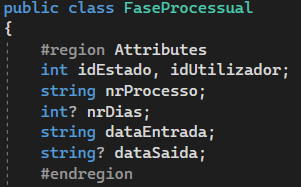
\includegraphics[width=0.5\textwidth]{Figuras/Models/FaseProcessualModel.png}
\caption{Fase Processual Model}
\label{d.model}
\end{figure}

\newpage
\indent \par Um utilizador pode criar uma fase processual, assim como alterar a sua data de saída. É também capaz de obter várias listagens de fases processuais, sendo elas, as fases processuais por número de processo,
por fase, assim como as ativas e inativas.
\indent \par Começamos então por testar a criação de uma fase processual e, em seguida, testamos a alteração da data final de uma fase processual. Ambos os testes de gestão de fases processuais tiveram sucesso.
\indent \par Por fim, testamos os quatro tipos de consulta de fases diferentes. Todos os testes obtiveram, também, resultado positivo.

\begin{figure}[!htbp]
  \centering
  \begin{minipage}[b]{0.4\textwidth}
    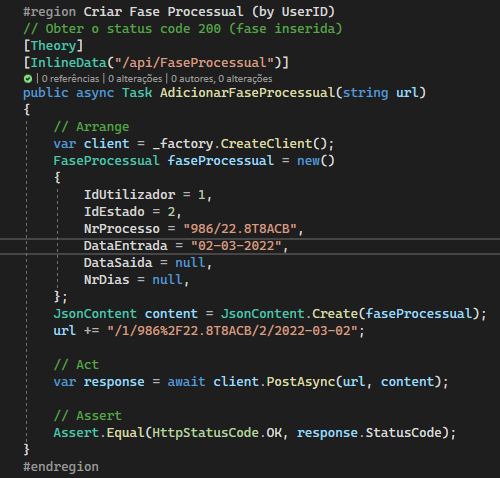
\includegraphics[width=\textwidth]{Figuras/TestesUnitarios/FaseProcessual/Criar Fase Processual.png}
    \caption{Criar Fase Processual (by UserID)}
    \label{d.unitario}
  \end{minipage}
  \hfill
  \begin{minipage}[b]{0.4\textwidth}
    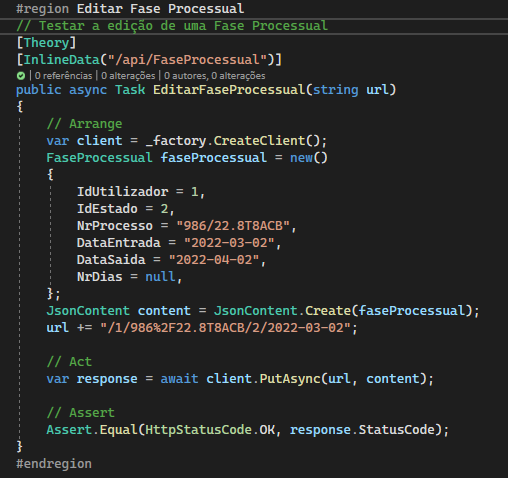
\includegraphics[width=\textwidth]{Figuras/TestesUnitarios/FaseProcessual/Editar Fase Processual.png}
    \caption{Editar Fase Processual (by UserID)}
    \label{d.unitario}
  \end{minipage}
  \centering
  \begin{minipage}[b]{0.4\textwidth}
    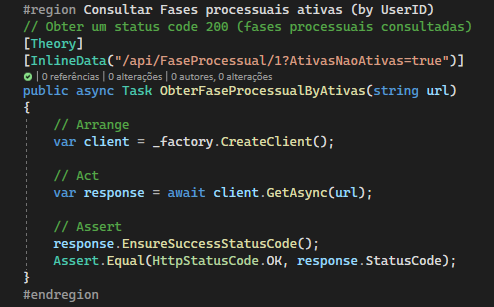
\includegraphics[width=\textwidth]{Figuras/TestesUnitarios/FaseProcessual/Consultar Fases Processuais Ativas.png}
    \caption{Consultar Fases Processuais Ativas (by UserID)}
    \label{d.unitario}
  \end{minipage}
  \hfill
  \begin{minipage}[b]{0.4\textwidth}
    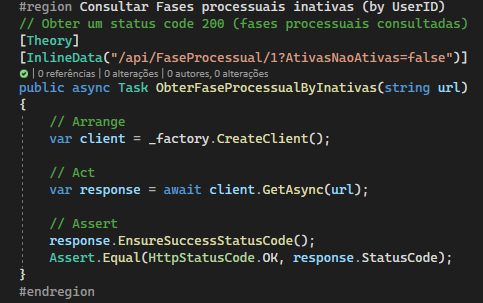
\includegraphics[width=\textwidth]{Figuras/TestesUnitarios/FaseProcessual/Consultar Fases Processuais Inativas.png}
    \caption{Consultar Fases Processuais Inativas (by UserID)}
    \label{d.unitario}
  \end{minipage}
  \centering
  \begin{minipage}[b]{0.4\textwidth}
    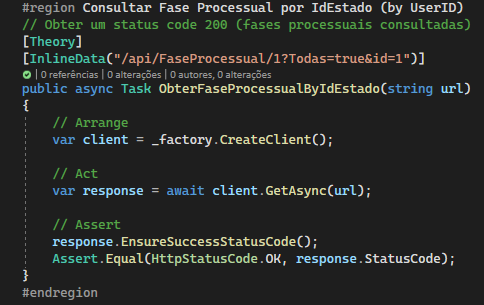
\includegraphics[width=\textwidth]{Figuras/TestesUnitarios/FaseProcessual/Consultar Fase Processual IdEstado.png}
    \caption{Consultar Fase Processual por IdEstado (by UserID)}
    \label{d.unitario}
  \end{minipage}
  \hfill
  \begin{minipage}[b]{0.4\textwidth}
    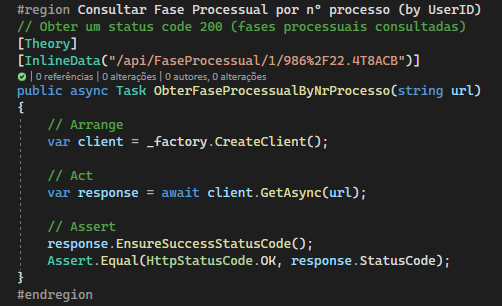
\includegraphics[width=\textwidth]{Figuras/TestesUnitarios/FaseProcessual/Consultar Fase Processual numero processo.png}
    \caption{Consultar Fase Processual por N° Processo (by UserID)}
    \label{d.unitario}
  \end{minipage}
\end{figure}

\begin{figure}[!tbp]
\centering
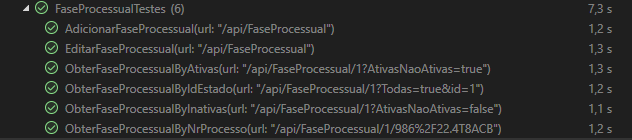
\includegraphics[width=1\textwidth]{Figuras/Testes/FaseProcessualTestes.png}
\caption{Fase Processual Testes}
\label{d.teste}
\end{figure}

\newpage


\subsection{Teste Unitário - Prazo Codigo}
\indent \par Para fazer a ligação entre os prazos e os códigos processuais, criamos o objeto Prazocodigo.
Este objeto é constituído pelos seguintes atributos:
\indent \par - Id - ID para identificação de um prazo código noutros objetos
\indent \par - IdTipoPrazo - ID para identificação do tipo de prazo
\indent \par - IdCodigo - ID para identificar o respetivo código processual existentes. O teste foi de encontro às expectativas.

\begin{figure}[!h]
\centering
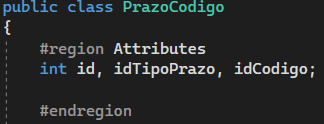
\includegraphics[width=0.6\textwidth]{Figuras/Models/PrazoCodigoModel.png}
\caption{Prazo Código Model}
\label{d.model}
\end{figure}

\indent \par O objetivo é armazenar os dados seguindo a seguinte estrutura genérica:
\indent \par - Prazo procedimental do código procedimento administrativo
\indent \par - Prazo de caducidade co código do processo civil
\indent \par - Prazo de caducidade do código do processo penal
\indent \par - Prazo processual do código do processo civil
\indent \par - Prazo processual do código do processo penal
\indent \par - Prazo de prescrição do código do processo civil
\indent \par - Prazo de prescrição do código do processo penal
\indent \par - Prazo de prescrição do regime ilicito de mera ordenação social

\indent \par Tendo em conta que apenas é necessária a listagem genérica, procedemos ao teste da sua obtenção. Este teste correu como o planeado.

\begin{figure}[!h]
\centering
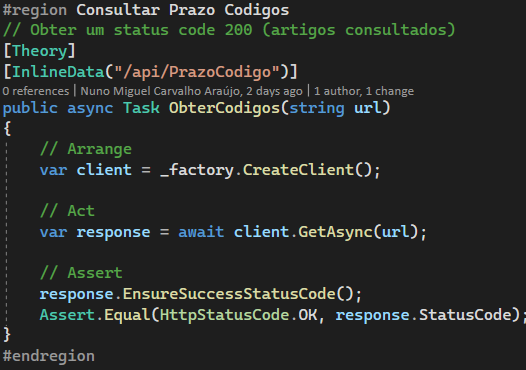
\includegraphics[width=0.4\textwidth]{Figuras/TestesUnitarios/PrazoCodigo/Consultar Prazo Códigos.png}
\caption{Consultar Prazo Códigos}
\label{d.unitario}
\end{figure}

\begin{figure}[!h]
\centering

\includegraphics[width=1\textwidth]{Figuras/Testes/PrazoCodigoTestes.png}
\caption{Prazo Código Testes}
\label{d.teste}
\end{figure}


\subsection{Teste Unitário - Prazo}
\indent \par Um processo tem sempre um prazo associado. Este prazo é calculado conforme o artigo que lhe for determinado. Cada artigo tem características singulares para o cálculo do prazo de um processo. Este cálculo é efetuado no prazo, e para isso, criamos uma estrutura com os seguintes atributos:
\indent \par - IdPrazoCodigo: ID para identificação do tipo de prazo do processo
\indent \par - IdUtilizador: ID para identificação do utilizador a que pertence o prazo
\indent \par - NrProcesso: Número de processo a que o prazo está associado
\indent \par - DataInicial: Data inicial definida para o prazo
\indent \par - DataFinal: Data final prevista para término do prazo, tendo em conta as características do artigo atribuído
\indent \par - NrArtigo: Identificação do artigo e respetivas características para cálculo do prazo (dias, meses, anos, dias úteis, férias, etc.)
\indent \par - IdCódigo: ID para identificação do tipo de código processual a que pertence o prazo

\begin{figure}[!h]
\centering
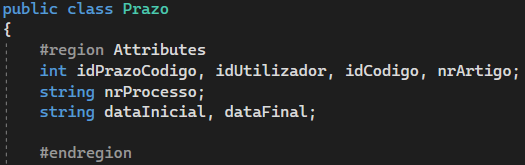
\includegraphics[width=0.6\textwidth]{Figuras/Models/PrazoModel.png}
\caption{Prazo Model}
\label{d.model}
\end{figure}

\newpage

\indent \par Um utilizador pode criar ou apagar um prazo, bem como consultar os prazos adicionados.
\indent \par Testamos a criação de um prazo pelo utilizador e o teste foi bem-sucedido. 
\indent \par Em seguida testamos a eliminação do prazo anteriormente criado. Este teste correu conforme o esperado.
\indent \par Por fim, testamos a consulta de todos os prazos de determinado utilizador, bem como os prazos por número de processo. Ambos os testes foram bem-sucedidos.

\begin{figure}[!htbp]
  \centering
  \begin{minipage}[b]{0.4\textwidth}
    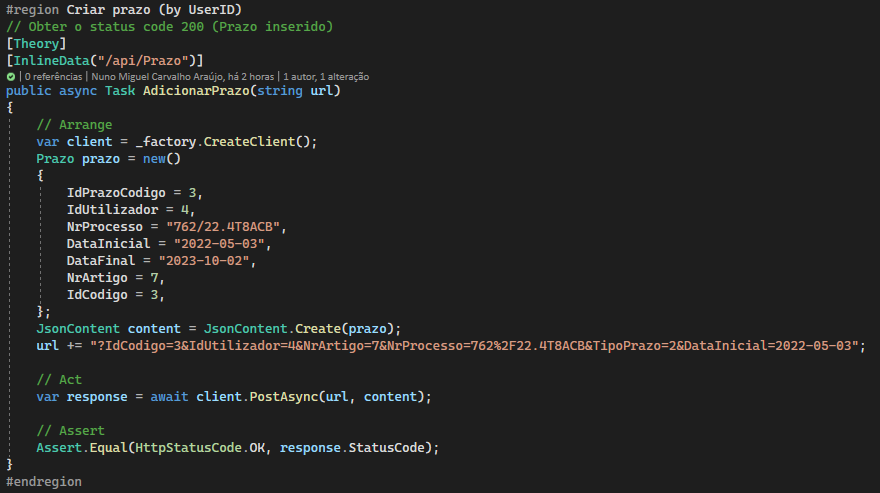
\includegraphics[width=\textwidth]{Figuras/TestesUnitarios/Prazo/Criar Prazo.png}
    \caption{Criar Prazo (by UserID)}
    \label{d.unitario}
  \end{minipage}
  \hfill
  \begin{minipage}[b]{0.4\textwidth}
    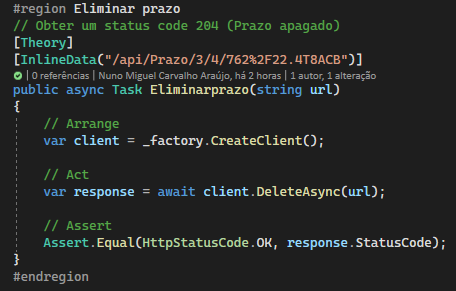
\includegraphics[width=\textwidth]{Figuras/TestesUnitarios/Prazo/Eliminar Prazo.png}
    \caption{Eliminar Prazo (by UserID)}
    \label{d.unitario}
  \end{minipage}
  \centering
  \begin{minipage}[b]{0.4\textwidth}
    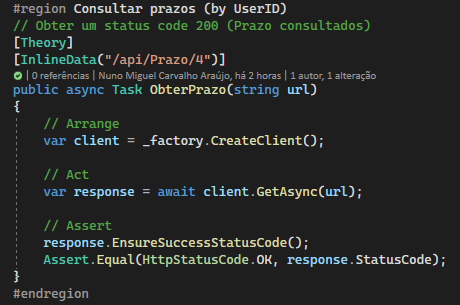
\includegraphics[width=\textwidth]{Figuras/TestesUnitarios/Prazo/Consultar Prazo (by UserID).png}
    \caption{Consultar Prazo (by UserID)}
    \label{d.unitario}
  \end{minipage}
  \hfill
  \begin{minipage}[b]{0.4\textwidth}
    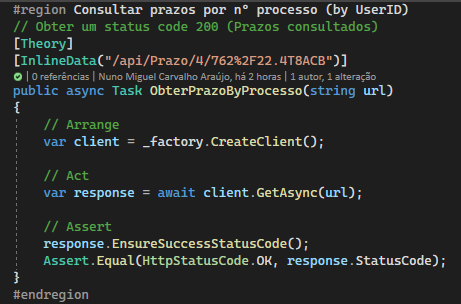
\includegraphics[width=\textwidth]{Figuras/TestesUnitarios/Prazo/Consultar Prazos por numero processo.png}
    \caption{Consultar Prazo por N°Processo (by UserID)}
    \label{d.unitario}
  \end{minipage}
\end{figure}

\begin{figure}[!h]
\centering
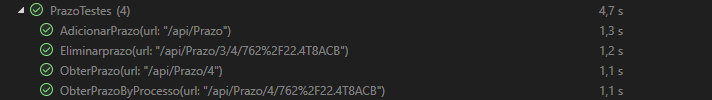
\includegraphics[width=1\textwidth]{Figuras/Testes/PrazoTestes.png}
\caption{Prazo Testes}
\label{d.teste}
\end{figure}


\subsection{Teste Unitário - Processo}
\indent \par O processo é um dos temas chave neste projeto. É necessário existir um processo para que lhe sejam atribuídos os mais variados campos pretendidos.
Assim sendo, criamos o processo com os seguintes atributos:
\indent \par - NrProcesso: Número de determinado processo
\indent \par - IdTipo: ID para identificação do tipo de processo
\indent \par - IdTema: ID para identificação do tema do processo
\indent \par - IdUtilizador: ID para identificação do utilizador a que o processo corresponde
\indent \par - Valor: Valor monetário envolvido no processo
\indent \par - Nome: Nome atribuído pelo utilizador ao processo
\indent \par - Notas: Comentários que o utilizador pretenda acrescentar ao processo
\indent \par - DataEntrada: Data de entrada do processo
\indent \par - Estado: Estado do processo. True se o processo estiver ativo, false caso contrário.

\begin{figure}[!h]
\centering
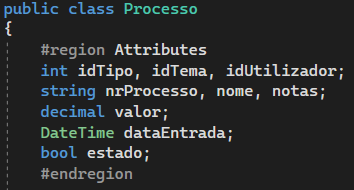
\includegraphics[width=0.4\textwidth]{Figuras/Models/ProcessoModel.png}
\caption{Processo Model}
\label{d.model}
\end{figure}

\indent \par Para cumprir com os objetivos delineados, começamos por testar a criação de um processo. Para isso, criamos uma instância de teste de um processo e tentamos fazer a sua adição. Este teste correu conforme o esperado.
\indent \par Em seguida, testamos a edição de um processo existente. Para isto, pegamos na instância de teste criada anteriormente e alteramos alguns campos. Mais uma vez, o teste ocorreu conforme as expectativas.
\indent \par Por fim, testamos a consulta de processos por utilizador. Esta consulta funciona sem problemas.

\begin{figure}[!htbp]
  \centering
  \begin{minipage}[b]{0.4\textwidth}
    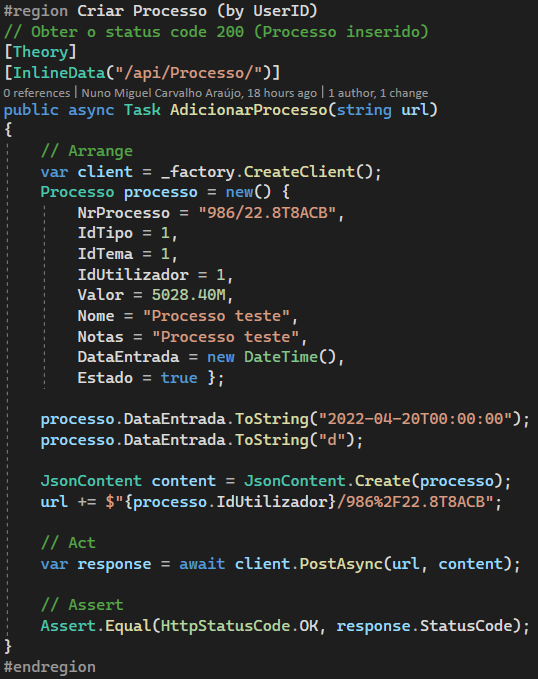
\includegraphics[width=\textwidth]{Figuras/TestesUnitarios/Processo/Criar Processo (by UserID).png}
    \caption{Criar Processo (by UserID)}
    \label{d.unitario}
  \end{minipage}
  \hfill
  \begin{minipage}[b]{0.4\textwidth}
    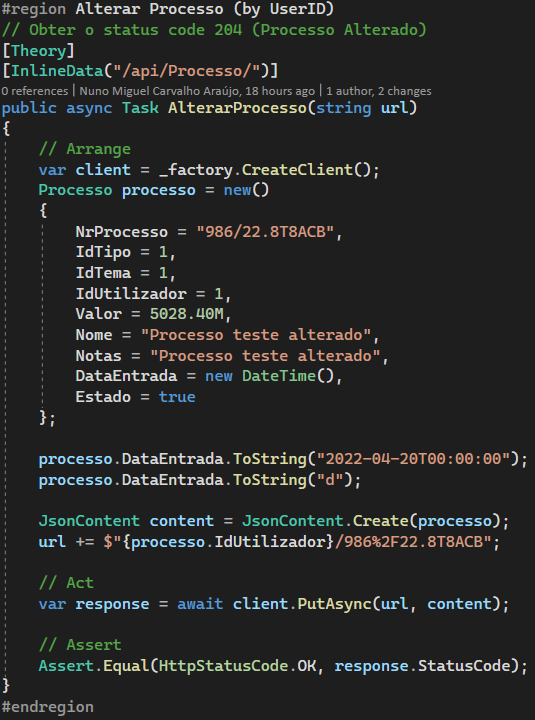
\includegraphics[width=\textwidth]{Figuras/TestesUnitarios/Processo/Alterar Processo (by User ID).png}
    \caption{Alterar Processo (by UserID)}
    \label{d.unitario}
  \end{minipage}
  \centering
  \begin{minipage}[b]{0.4\textwidth}
    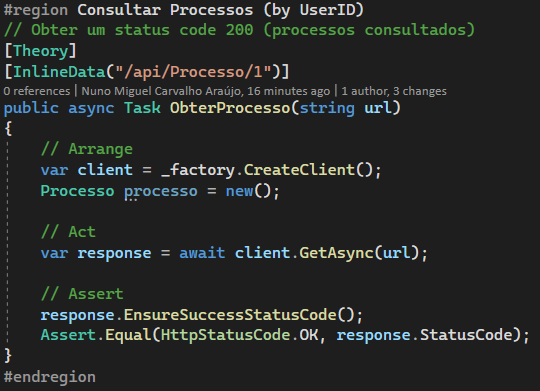
\includegraphics[width=\textwidth]{Figuras/TestesUnitarios/Processo/Consultar Processo (by User ID).png}
    \caption{Consultar Processo (by UserID)}
    \label{d.unitario}
  \end{minipage}
\end{figure}

\begin{figure}[!h]
\centering
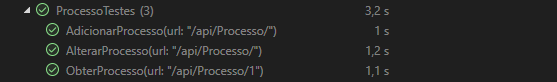
\includegraphics[width=1\textwidth]{Figuras/Testes/ProcessoTestes.png}
\caption{Processo Testes}
\label{d.teste}
\end{figure}

\newpage


\subsection{Teste Unitário - Tema}
\indent \par Cada processo tem o seu tipo e, dentro desse tipo, está atribuído um tema. Assim sendo, criamos o Tema com os seguintes atributos:
\indent \par - Id: ID para identificação do tema 
\indent \par - IdUtilziador: ID para identificação do utilizador a que pertence o tema
\indent \par - Nome: Nome atribuído ao tema, pelo utilizador

\begin{figure}[!h]
\centering
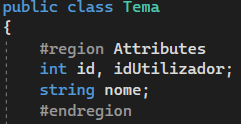
\includegraphics[width=0.4\textwidth]{Figuras/Models/TemaModel.png}
\caption{Tema Model}
\label{d.model}
\end{figure}

\indent \par Em relação aos casos de uso, determinamos que cada utilizador poderia inserir um tema, alterar um tema ou consultar todos os temas por ele inseridos.
\indent \par Criamos, então, uma instância teste de um tema para proceder à sua inserção. O teste foi executado com sucesso.
\indent \par Em seguida, modificamos a instância criada anteriormente para testar a sua alteração. Este teste também teve sucesso.
\indent \par Por fim, testamos a consulta de temas inseridos por utilizador, obtendo novamente resultado positivo.

\begin{figure}[!htbp]
  \centering
  \begin{minipage}[b]{0.4\textwidth}
    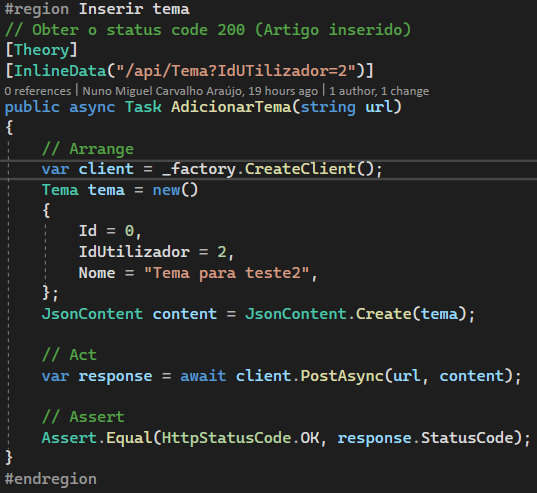
\includegraphics[width=\textwidth]{Figuras/TestesUnitarios/Tema/Inserir Tema.png}
    \caption{Inserir Tema}
    \label{d.unitario}
  \end{minipage}
  \hfill
  \begin{minipage}[b]{0.4\textwidth}
    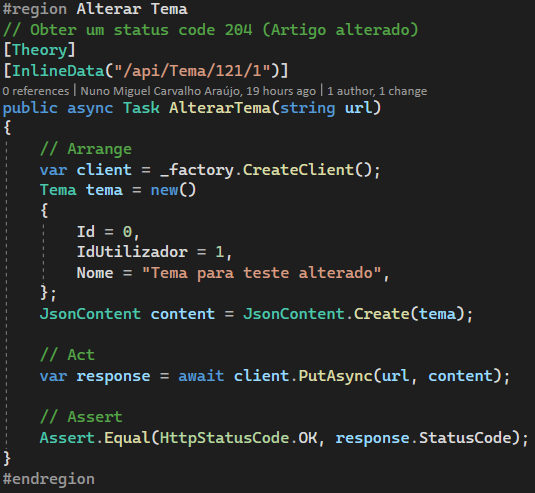
\includegraphics[width=\textwidth]{Figuras/TestesUnitarios/Tema/Alterar Tema.png}
    \caption{Alterar Tema}
    \label{d.unitario}
  \end{minipage}
  \centering
  \begin{minipage}[b]{0.4\textwidth}
    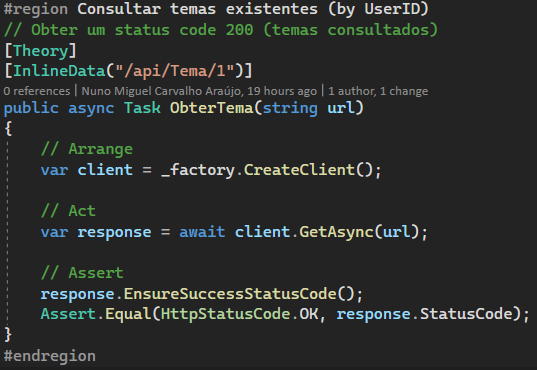
\includegraphics[width=\textwidth]{Figuras/TestesUnitarios/Tema/Consultar temas existentes (by User ID).png}
    \caption{Consultar Temas (by UserID)}
    \label{d.unitario}
  \end{minipage}
\end{figure}

\begin{figure}[!tbp]
\centering

\includegraphics[width=1\textwidth]{Figuras/Testes/TemaTestes.png}
\caption{Tema Testes}
\label{d.teste}
\end{figure}

\newpage


\subsection{Teste Unitário - Tipo Prazo}
\indent \par Assim como o Código, o tipo de prazo armazena uma listagem genérica de tipos de prazo de um processo. Sendo assim, criamos o tipo de prazo com os seguintes atributos:
\indent \par - Id: ID para a identificação do tipo de prazo noutros objetos
\indent \par - Nome: Discriminação de um tipo de prazo (Prazo procedimental, prazo de caducidade, prazo processual e prazo de prescrição)

\begin{figure}[!h]
\centering
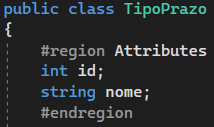
\includegraphics[width=0.4\textwidth]{Figuras/Models/TipoPrazoModel.png}
\caption{Tipo Prazo Model}
\label{d.model}
\end{figure}

\indent \par Sendo uma listagem genérica, apenas testamos a obtenção da lista dos tipos de prazo existentes. O teste foi de encontro às expectativas.

\begin{figure}[!h]
\centering
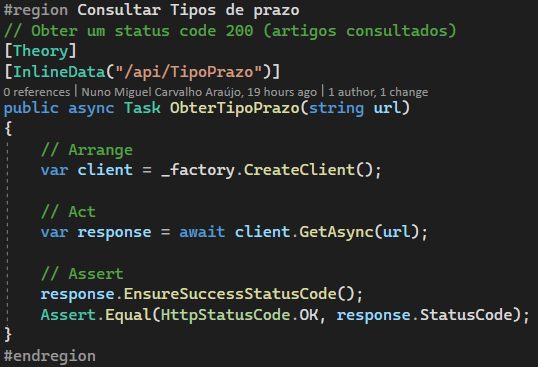
\includegraphics[width=0.4\textwidth]{Figuras/TestesUnitarios/TipoPrazo/Consultar Tipos de prazo.png}
\caption{Consultar Tipos de Prazo}
\label{d.unitario}
\end{figure}

\begin{figure}[!h]
\centering

\includegraphics[width=1\textwidth]{Figuras/Testes/TipoPrazoTestes.png}
\caption{Tipo Prazo Testes}
\label{d.teste}
\end{figure}


\subsection{Teste Unitário - Tipo Processo}
\indent \par Como referido anteriormente, cada processo tem o seu tipo e, a cada tipo, está um tema associado. O tipo de processo deve ser inserido a gosto do utilizador, mas terá, sempre um tema associado. Desta forma, criamos o tipo de processo com os seguintes atributos:
\indent \par - Id: ID para identificação do tipo de processo noutros objetos
\indent \par - IdUtilizador: ID para identificação do utilizador a que pertence o tipo de prazo
\indent \par - Nome: Nome atribuído ao tipo de processo, pelo utilizador
\indent \par - IdTema: ID do tema associado ao tipo de processo

\begin{figure}[!h]
\centering
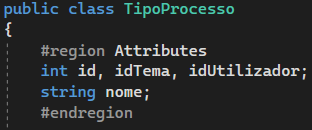
\includegraphics[width=0.6\textwidth]{Figuras/Models/TipoProcessoModel.png}
\caption{Tipo Processo Model}
\label{d.model}
\end{figure}


\indent \par Para corresponder com os objetivos delineados, é necessário um utilizador poder criar um tipo de processo assim como alterá-lo.
\indent \par Para testar a criação de um tipo de processo, criamos uma instância de um tipo de processo e procedemos à implementação. O resultado do teste foi satisfatório.
\indent \par Por fim, testamos a alteração de campos da instância criada anteriormente. Obtemos, também, um resultado positivo neste teste.

\begin{figure}[!htbp]
  \centering
  \begin{minipage}[b]{0.4\textwidth}
    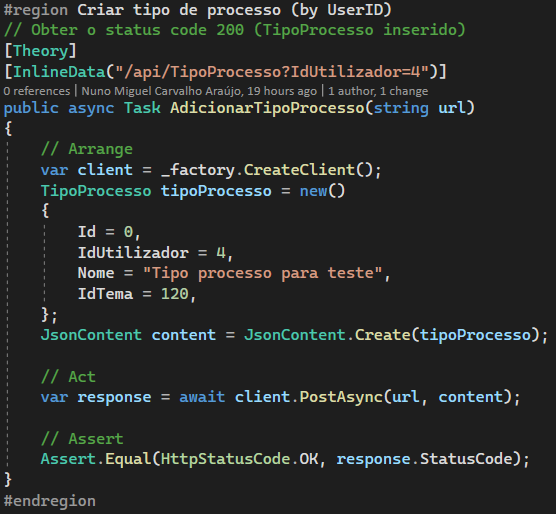
\includegraphics[width=\textwidth]{Figuras/TestesUnitarios/TipoProcesso/Criar tipo de processo (by UserID).png}
    \caption{Criar Tipo de Processo (by UserID)}
    \label{d.unitario}
  \end{minipage}
  \hfill
  \begin{minipage}[b]{0.4\textwidth}
    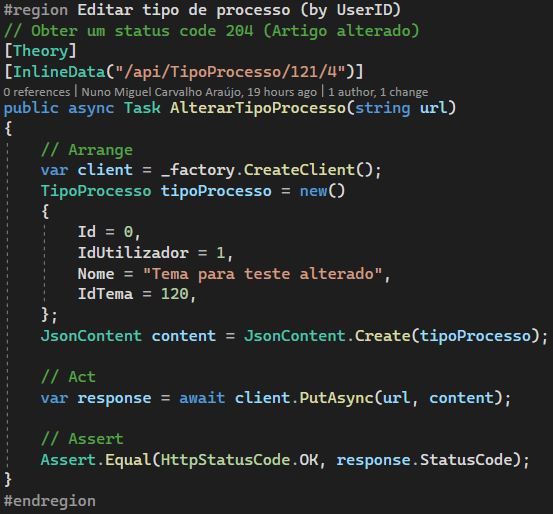
\includegraphics[width=\textwidth]{Figuras/TestesUnitarios/TipoProcesso/Editar tipo de processo (by UserID).png}
    \caption{Editar Tipo de Processo (by UserID)}
    \label{d.unitario}
  \end{minipage}
\end{figure}

\begin{figure}[!h]
\centering
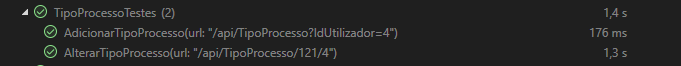
\includegraphics[width=1\textwidth]{Figuras/Testes/TipoProcessoTestes.png}
\caption{Tipo Processo Testes}
\label{d.teste}
\end{figure}

\newpage


\subsection{Teste Unitário - Utilizador}
\indent \par Na nossa perspetiva, um utilizador é um cliente do nosso serviço. Um cliente é constituído pelos seguintes atributos:
\indent \par - Id: ID para identificação do utilizador noutros objetos
\indent \par - Nome: Nome do utilizador
\indent \par - Email: Email do utilizador, necessário para acesso à plataforma e para a receção de notificações à cerca dos prazos
\indent \par - Password: Senha de acesso ao portal

\begin{figure}[!h]
\centering
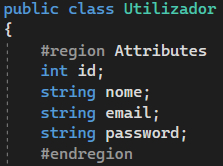
\includegraphics[width=0.3\textwidth]{Figuras/Models/UtilizadorModel.png}
\caption{Utilizador Model}
\label{d.model}
\end{figure}

\newpage

\indent \par Neste projeto, o utilizador é o principal interveniente. Ele tem permissões para criar conta com um email que ainda não esteja associado, bem como alterar os dados da sua conta.
\indent \par Criamos então um utilizador de exemplo para testar o seu sign up. O resultado do teste foi positivo.
\indent \par Em seguida, alteramos dados do utilizador criado anteriormente e testamos. O resultado obtido foi, novamente, satisfatório.

\begin{figure}[!htbp]
  \centering
  \begin{minipage}[b]{0.4\textwidth}
    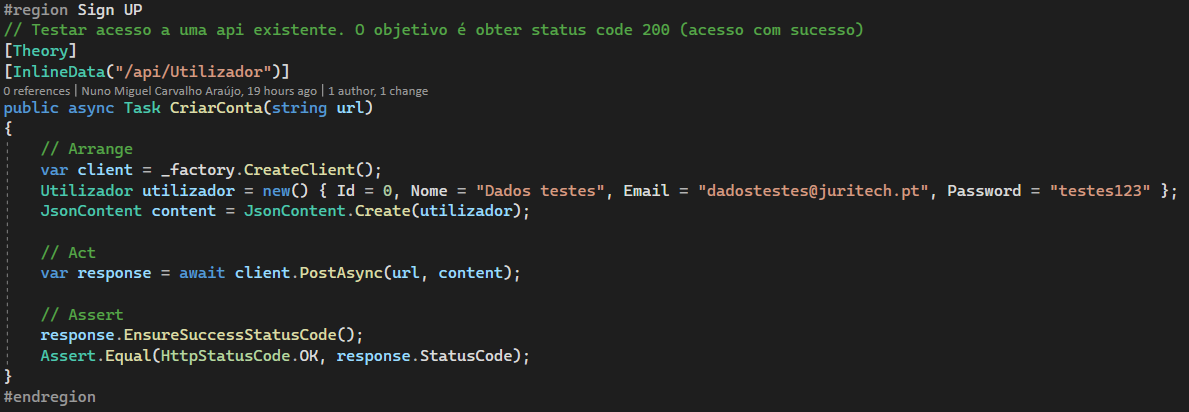
\includegraphics[width=\textwidth]{Figuras/TestesUnitarios/Utilizador/Sign UP.png}
    \caption{Sign Up}
    \label{d.unitario}
  \end{minipage}
  \hfill
  \begin{minipage}[b]{0.4\textwidth}
    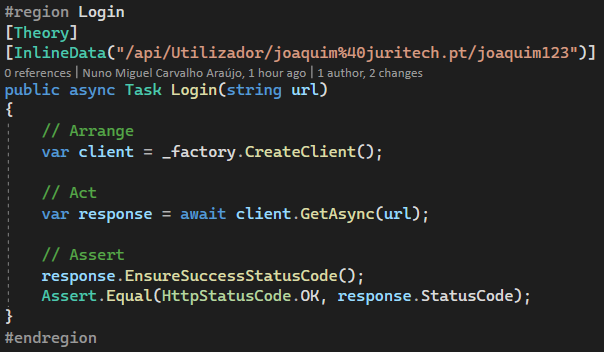
\includegraphics[width=\textwidth]{Figuras/TestesUnitarios/Utilizador/Login.png}
    \caption{Login}
    \label{d.unitario}
  \end{minipage}
  \centering
  \begin{minipage}[b]{0.4\textwidth}
    \includegraphics[width=\textwidth]{Figuras/TestesUnitarios/Utilizador/Editar dados de utilizador.png}
    \caption{Editar Dados de Utilizador}
    \label{d.unitario}
  \end{minipage}
\end{figure}

\begin{figure}[!h]
\centering
\includegraphics[width=1\textwidth]{Figuras/Testes/UtilizadorTestes.png}
\caption{Utilizador Testes}
\label{d.teste}
\end{figure}

\newpage


\subsection{Bugs Conhecidos}
\indent \par Neste momento, as notificações para o utilizador ainda não estão implementadas. Temos consciência que as notificações via email são uma das funcionalidades mais importantes no projeto, no entanto, ainda não tivemos a possibilidade de as implementar. Esperamos resolver este problema o mais rapidamente possível.
\indent \par Após a implementação das notificações, pretendemos possibilitar também ao utilizador a recuperação da sua password através do email. Supomos que ambas as funcionalidades tenham parecenças, por isso, pretendemos implementar as notificações e a recuperação de senhas simultaneamente.
\indent \par É possível que existam também alguns bugs e falhas de verificações de campos.
Durante a execução dos testes unitários, fomos encontrando alguns e procedemos à sua resolução. No entanto, estamos preparados para encontrar mais conforme vamos experimentando o projeto.  
